\documentclass[border=10pt]{standalone}
\usepackage{tikz}
\usetikzlibrary{arrows.meta}

\begin{document}
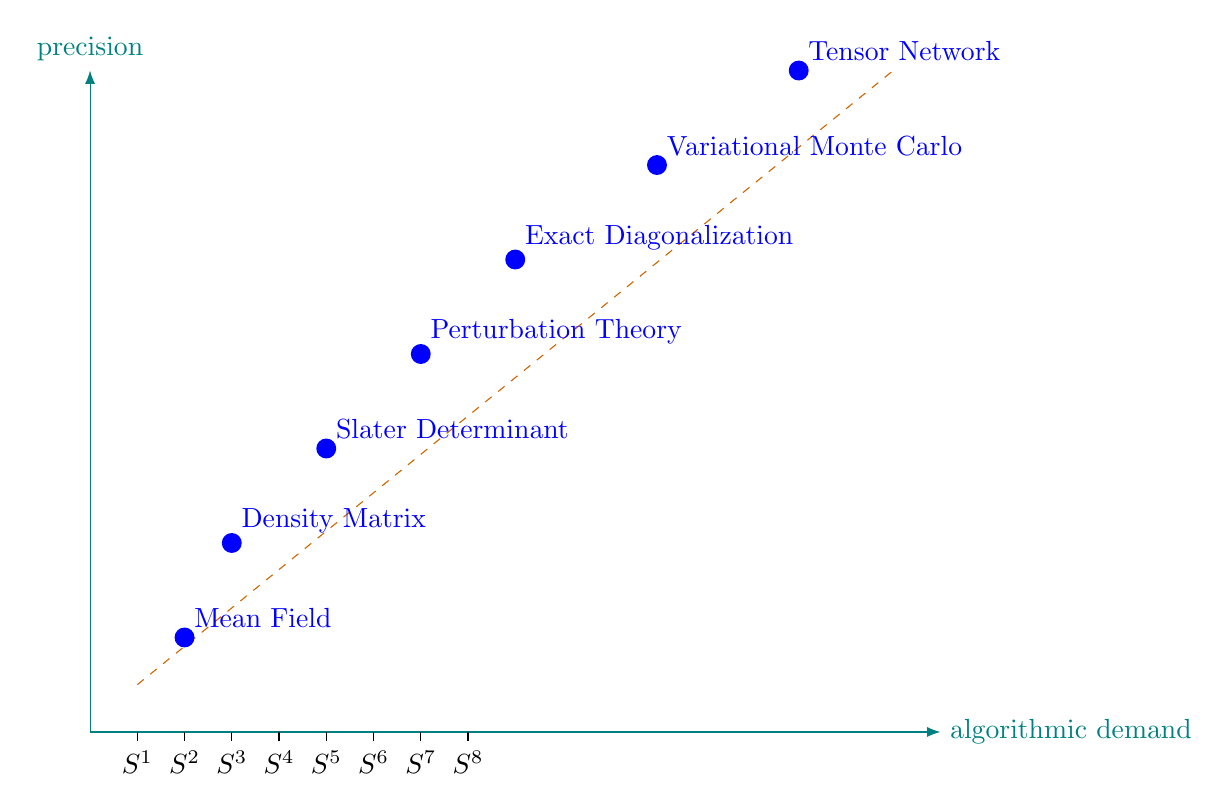
\begin{tikzpicture}[scale=1.2]

% Axes
\draw[-Latex, teal] (0,0) -- (9,0) node[right] {algorithmic demand};
\draw[-Latex, teal] (0,0) -- (0,7) node[above] {precision};

% Tick Marks and Labels
\foreach \x [evaluate=\x as \label using int(\x)] in {1,...,8} {
    \draw (0.5*\x, 0) -- ++(0,-0.1) node[below] {$S^\x$};
}

% Trend Line
\draw[dashed, orange!80!black] (0.5,0.5) -- (8.5,7);

% Data Points and Annotations
\foreach \method/\x/\y in {
    Mean Field/1/1,
    Density Matrix/1.5/2,
    Slater Determinant/2.5/3,
    Perturbation Theory/3.5/4,
    Exact Diagonalization/4.5/5,
    Variational Monte Carlo/6/6,
    Tensor Network/7.5/7
}{
    \fill[blue] (\x,\y) circle (3pt);
    \node[anchor=south west, blue] at (\x,\y) {\method};
}

\end{tikzpicture}
\end{document}